\documentclass[aspectratio=169, 9pt]{beamer}

% ── Theme ─────────────────────────────────────────────────────────────────────
\usetheme{Madrid}
\usecolortheme{default}
\setbeamertemplate{navigation symbols}{}
\setbeamertemplate{footline}[frame number]

% ── Fonts & encoding ──────────────────────────────────────────────────────────
\usepackage[T1]{fontenc}
\usepackage[utf8]{inputenc}
\usepackage{lmodern}

% ── Math ──────────────────────────────────────────────────────────────────────
\usepackage{amsmath, amssymb}

% ── Tables ────────────────────────────────────────────────────────────────────
\usepackage{booktabs}
\usepackage{tabularx}
\usepackage{array}

% ── Graphics ──────────────────────────────────────────────────────────────────
\usepackage{tikz}
\usetikzlibrary{arrows.meta, positioning, shapes.geometric, fit, backgrounds}

% ── Misc ──────────────────────────────────────────────────────────────────────
\usepackage{microtype}
\usepackage{enumitem}
\usepackage{xcolor}

% ── Color palette ─────────────────────────────────────────────────────────────
\definecolor{navyblue}{HTML}{1A237E}
\definecolor{medblue}{HTML}{1565C0}
\definecolor{teal}{HTML}{00695C}
\definecolor{purple}{HTML}{6A1B9A}
\definecolor{orange}{HTML}{E65100}
\definecolor{darkred}{HTML}{B71C1C}
\definecolor{darkgreen}{HTML}{1B5E20}
\definecolor{lightgray}{HTML}{F5F5F5}
\definecolor{warnorange}{HTML}{E65100}
\definecolor{warnbg}{HTML}{FFF3E0}

% ── Beamer colors ─────────────────────────────────────────────────────────────
\setbeamercolor{frametitle}{bg=navyblue, fg=white}
\setbeamercolor{title}{fg=white}
\setbeamercolor{author}{fg=white}
\setbeamercolor{date}{fg=white}
\setbeamercolor{structure}{fg=navyblue}
\setbeamercolor{titlelike}{bg=navyblue}
\setbeamercolor{palette primary}{bg=navyblue, fg=white}
\setbeamercolor{palette secondary}{bg=medblue, fg=white}
\setbeamercolor{palette tertiary}{bg=navyblue!80, fg=white}

% ── Custom block colors ───────────────────────────────────────────────────────
\setbeamercolor{block title}{bg=navyblue, fg=white}
\setbeamercolor{block body}{bg=lightgray, fg=black}
\setbeamercolor{alertblock title}{bg=darkred, fg=white}
\setbeamercolor{alertblock body}{bg=darkred!8, fg=black}
\setbeamercolor{exampleblock title}{bg=teal, fg=white}
\setbeamercolor{exampleblock body}{bg=teal!8, fg=black}

% ── Helper: colored pill badge ────────────────────────────────────────────────
\newcommand{\badge}[2]{%
  \tikz[baseline=(n.base)]\node[fill=#1, text=white,
    rounded corners=3pt, inner sep=3pt, font=\scriptsize\bfseries](n){#2};}

% ─────────────────────────────────────────────────────────────────────────────
\title[DermAtlas ML Pipeline]{\textbf{DermAtlas}\\Clinical Decision Support for Dermatology}
\subtitle{ML Pipeline --- Progress Presentation}
\author{DermAtlas Team}
\date{}

% ─────────────────────────────────────────────────────────────────────────────
\begin{document}

\begin{frame}
  \titlepage
\end{frame}

% ═════════════════════════════════════════════════════════════════════════════
% SLIDE A — The Problem
% ═════════════════════════════════════════════════════════════════════════════
\begin{frame}{Slide 1 --- The Problem: A Critical Gap in Dermatologic Care}

  \begin{columns}[T]

    \begin{column}{0.48\textwidth}
      \begin{alertblock}{Survival Rates Drop Dramatically}
        \small
        Skin cancer caught in \textbf{early stages} has a survival
        rate of nearly \textbf{100\%}. By advanced stages, that
        number falls to around \textbf{30\%}. Early diagnosis is
        not a convenience --- it is the difference between life
        and death.
      \end{alertblock}

      \vspace{0.4em}
      \begin{alertblock}{Supply Cannot Meet Demand}
        \small
        Tens of millions of dermatology-related visits occur each
        year, but the number of dermatologists is severely limited.
        The result: \textbf{wait times of over a month} for a
        specialist appointment --- far too long when a lesion
        may be malignant.
      \end{alertblock}
    \end{column}

    \begin{column}{0.48\textwidth}
      \begin{block}{The Uncertainty Gap}
        \small
        Primary care physicians handle the majority of initial
        skin evaluations. But dermatologic diagnosis is
        \textbf{highly visual and pattern-based} --- requiring
        specialized expertise most PCPs simply do not have.
        This creates a critical uncertainty gap:
        \begin{itemize}[leftmargin=1em, itemsep=2pt]
          \item Delayed diagnoses
          \item Unnecessary referrals
          \item Strained healthcare resources
          \item Loss of the early-stage treatment window
        \end{itemize}
      \end{block}

      \vspace{0.4em}
      \begin{exampleblock}{The Question}
        \small
        \textbf{What if this gap could be eliminated?} A solution
        that enables instant, specialist-level triage could reduce
        diagnostic delays to zero and empower every primary care
        physician to make fast, accurate, and confident decisions.
      \end{exampleblock}
    \end{column}

  \end{columns}

\end{frame}

% ═════════════════════════════════════════════════════════════════════════════
% SLIDE B — The Solution: DermAtlas
% ═════════════════════════════════════════════════════════════════════════════
\begin{frame}{Slide 2 --- DermAtlas: The Solution}

  \begin{columns}[T]

    \begin{column}{0.48\textwidth}
      \textbf{\color{navyblue}What DermAtlas Is}

      \vspace{0.3em}
      {\small
      DermAtlas is a \textbf{clinical decision support system}
      designed to give primary care physicians instant,
      explainable, specialist-level triage at the point of care.
      A physician captures or uploads a lesion image; DermAtlas
      returns a malignancy assessment alongside visually similar
      expert-labeled historical cases --- so the physician
      understands \textit{why}, not just \textit{what}.
      }

      \vspace{0.4em}
      \begin{exampleblock}{Human-in-the-Loop}
        \small
        DermAtlas \textbf{augments} the physician --- it never
        makes the final call. Every prediction is explainable,
        every decision belongs to the clinician.
      \end{exampleblock}
    \end{column}

    \begin{column}{0.48\textwidth}
      \textbf{\color{navyblue}System Architecture}

      \vspace{0.3em}
      \begin{block}{Backend}
        \small
        \begin{itemize}[leftmargin=1em, itemsep=2pt]
          \item Cloud-hosted on \textbf{GCP} (Cloud Run, Cloud SQL,
            Cloud Storage)
          \item \textbf{Relational database} storing cases, metadata,
            and physician feedback
          \item \textbf{Role-based access control} with service-account
            isolation --- HIPAA-aligned
          \item ML pipeline: embedding \& classification \textbf{(built)};
            vector search \& Bayesian update layer \textbf{(in progress)}
        \end{itemize}
      \end{block}

      \vspace{0.3em}
      \begin{block}{Frontend}
        \small
        \begin{itemize}[leftmargin=1em, itemsep=2pt]
          \item \textbf{Cross-platform React Native} (Expo) app
          \item Physician captures or uploads lesion image
          \item Side-by-side display of retrieved similar cases
          \item Malignancy score with confidence and class distribution
        \end{itemize}
      \end{block}
    \end{column}

  \end{columns}

\end{frame}

% ═════════════════════════════════════════════════════════════════════════════
% SLIDE 1 — Data Sources
% ═════════════════════════════════════════════════════════════════════════════
\begin{frame}{Slide 3 --- Building the Training Dataset}

  \begin{columns}[T]

    %% ── Left: three dataset cards ──────────────────────────────────────────
    \begin{column}{0.48\textwidth}
      \textbf{\color{navyblue}Why these three datasets?}\\[0.4em]
      The largest publicly available, histologically confirmed dermoscopy collections.
      Together they cover all 6 target classes.

      \vspace{0.6em}
      \begin{block}{HAM10000}
        \small 9,873 images · Vienna \& Brisbane\\
        Histologically confirmed · 6 classes
      \end{block}

      \vspace{0.3em}
      \begin{block}{ISIC 2019}
        \small 14,774 images · Multi-center\\
        6-class labeled · international cohort
      \end{block}

      \vspace{0.3em}
      \begin{block}{ISIC 2020}
        \small 33,126 images · Multi-center\\
        \textasciitilde6,000 labeled · 27,126 unknown benign
      \end{block}

      \vspace{0.5em}
      \textbf{Output:} \texttt{unified\_metadata.csv}\\
      {\small 57,773 rows · 13 columns}
    \end{column}

    %% ── Right: metadata schema + shortcomings ──────────────────────────────
    \begin{column}{0.48\textwidth}
      \textbf{\color{navyblue}Unified metadata columns}

      \vspace{0.3em}
      {\small
      \begin{tabular}{@{} ll @{}}
        \toprule
        Column & Description \\
        \midrule
        \texttt{image\_id}       & Unique image ID \\
        \texttt{source\_dataset} & ham10000 / isic2019 / isic2020 \\
        \texttt{mel, nv, bcc}   & Class label (0/1) \\
        \texttt{akiec, bkl, df} & Class label (0/1) \\
        \texttt{age, sex}       & Patient demographics \\
        \texttt{localization}   & Body site \\
        \texttt{malignant}      & Derived binary label \\
        \bottomrule
      \end{tabular}
      }

      \vspace{0.6em}
      \begin{alertblock}{Shortcomings}
        \small
        \begin{itemize}[leftmargin=1em, itemsep=0pt]
          \item \textbf{Class imbalance} --- only 9,493 malignant vs 48,280 benign
          \item \textbf{Skin tone bias} --- predominantly light-skinned European / Australian patients
          \item \textbf{Rare classes} --- df: 239 samples · akiec: 1,064 samples
          \item \textbf{Potential duplicates} --- ISIC 2019 \& 2020 share image sources
        \end{itemize}
      \end{alertblock}
    \end{column}

  \end{columns}
\end{frame}

% ═════════════════════════════════════════════════════════════════════════════
% SLIDE 6 (moved) — Dataset Details
% ═════════════════════════════════════════════════════════════════════════════
\begin{frame}{Slide 4 --- Dataset Details: Class Distribution \& Split}

  \begin{columns}[T]

    %% ── Left: class distribution table ─────────────────────────────────────
    \begin{column}{0.54\textwidth}
      \textbf{\color{navyblue}Class Distribution (30,647 labeled rows)}

      \vspace{0.3em}
      {\small
      \begin{tabular}{@{} l r r r @{}}
        \toprule
        Class & Count & \% labeled & MLP weight \\
        \midrule
        {\color{teal}nv}    & 18,068 & 58.9\% & 0.249 \\
        {\color{orange}mel} &  5,106 & 16.7\% & 0.881 \\
        {\color{orange}bcc} &  3,323 & 10.8\% & 1.354 \\
        {\color{teal}bkl}   &  2,847 &  9.3\% & 1.581 \\
        {\color{orange}akiec} & 1,064 & 3.5\% & 4.231 \\
        {\color{teal}df}    &    239 &  0.8\% & 18.85 \\
        \midrule
        {\color{darkred}Malignant} & 9,493 & 31.0\% & \\
        {\color{darkgreen}Benign}  & 21,154 & 69.0\% & \\
        \bottomrule
      \end{tabular}
      }

      \vspace{0.4em}
      {\scriptsize\color{gray}
      Inverse class-frequency weights ($w_c \propto 1/N_c$) applied to CrossEntropyLoss.\\
      75:1 nv:df imbalance makes weighting essential.}
    \end{column}

    %% ── Right: source breakdown + train/test split ──────────────────────────
    \begin{column}{0.42\textwidth}
      \textbf{\color{navyblue}Source Breakdown}

      \vspace{0.3em}
      {\small
      \begin{tabular}{@{} l r r @{}}
        \toprule
        Dataset & Images & Labeled \\
        \midrule
        HAM10000  &  9,873 &  9,873 \\
        ISIC 2019 & 14,774 & 14,774 \\
        ISIC 2020 & 33,126 &  6,000 \\
        \midrule
        \textbf{Total} & \textbf{57,773} & \textbf{30,647} \\
        \bottomrule
      \end{tabular}
      }

      \vspace{0.5em}
      \textbf{\color{navyblue}Train / Test Split}

      \vspace{0.3em}
      {\small
      \begin{tabular}{@{} l r r r @{}}
        \toprule
        Split & Rows & Mal. & Ben. \\
        \midrule
        Train 75\% & 22,985 & 7,120 & 15,865 \\
        Test  25\% &  7,662 & 2,373 &  5,289 \\
        \bottomrule
      \end{tabular}
      }

      \vspace{0.4em}
      {\scriptsize\color{gray}
      Stratified once, locked.\\ All downstream models respect this boundary.}
    \end{column}

  \end{columns}
\end{frame}

% ═════════════════════════════════════════════════════════════════════════════
% SLIDE 2 — Embedding Generation
% ═════════════════════════════════════════════════════════════════════════════
\begin{frame}{Slide 5 --- Turning Images into Numbers}

  \begin{columns}[T]

    %% ── Left: why Vertex AI ───────────────────────────────────────────────
    \begin{column}{0.50\textwidth}
      \textbf{\color{navyblue}Why Vertex AI Embeddings?}

      \vspace{0.4em}
      Images are unstructured --- ML models need fixed-size numeric vectors.
      Vertex AI \texttt{multimodalembedding@001} gives us exactly that.

      \vspace{0.5em}
      \begin{exampleblock}{What it does}
        \small
        \begin{itemize}[leftmargin=1em, itemsep=0pt]
          \item Vision Transformer (ViT) backbone
          \item Produces a \textbf{1408-D float32 vector} per image
          \item Captures texture, color, shape globally
          \item No GPU infrastructure needed on our end --- pure API call
          \item 57,773 images embedded at 600 req/min via GCS pipeline
        \end{itemize}
      \end{exampleblock}

      \vspace{0.5em}
      \textbf{\color{navyblue}Stored on GCS:}\\[0.3em]
      {\small
      \begin{tabular}{@{} ll @{}}
        \texttt{embeddings.npy} & (57773 $\times$ 1408) \\
        \texttt{labels.npy}     & (57773 $\times$ 6) \\
        \texttt{image\_ids.npy} & (57773,) \\
      \end{tabular}
      }
    \end{column}

    %% ── Right: limitation + future work ───────────────────────────────────
    \begin{column}{0.46\textwidth}

      \begin{alertblock}{Key Limitation}
        \small
        \texttt{multimodalembedding@001} was trained on \textbf{general internet
        images}, not dermoscopy. It may miss domain-specific structures:
        \begin{itemize}[leftmargin=1em, itemsep=0pt]
          \item Blue--white veils
          \item Regression areas
          \item Milia-like cysts
          \item Dermoscopic pigment networks
        \end{itemize}
      \end{alertblock}

      \vspace{0.6em}
      \begin{block}{Next Steps}
        \small
        For the next deadline we are evaluating a switch to a
        \textbf{dermoscopy-specific foundation model}
        (e.g.\ SkinGPT, DermFoundation).
        Domain-specific pretraining would produce richer embeddings
        and is expected to improve downstream classifier performance
        --- especially for rare classes like df and akiec.
      \end{block}

    \end{column}

  \end{columns}
\end{frame}

% ═════════════════════════════════════════════════════════════════════════════
% SLIDE 3 — ML Pipeline Overview
% ═════════════════════════════════════════════════════════════════════════════
\begin{frame}{Slide 6 --- ML Pipeline Overview}

  \vspace{0.3em}
  \begin{center}
  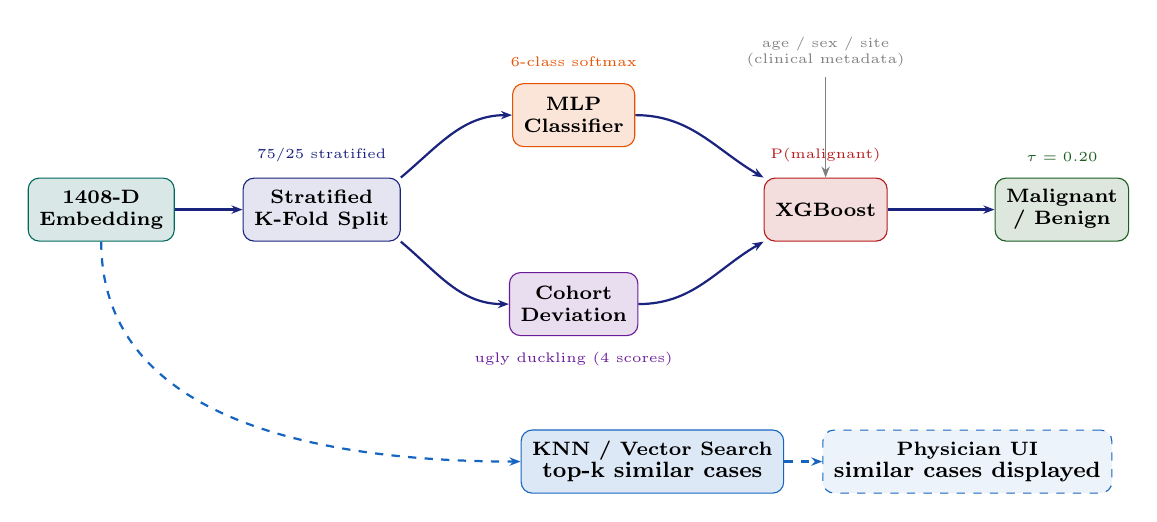
\begin{tikzpicture}[
    box/.style  = {draw, rounded corners=4pt, align=center,
                   font=\scriptsize\bfseries, inner sep=4pt, minimum height=0.8cm},
    arr/.style  = {-{Stealth[length=4pt]}, thick, color=navyblue},
    parr/.style = {-{Stealth[length=4pt]}, thick, dashed, color=medblue},
  ]

    %% ── Main nodes ──────────────────────────────────────────────────────────
    \node[box, fill=teal!15,      draw=teal]       (emb)    at (0,    0)   {1408-D\\Embedding};
    \node[box, fill=navyblue!12,  draw=navyblue]   (split)  at (2.8,  0)   {Stratified\\K-Fold Split};
    \node[box, fill=orange!15,    draw=orange]     (mlp)    at (6.0,  1.2) {MLP\\Classifier};
    \node[box, fill=purple!15,    draw=purple]     (cohort) at (6.0, -1.2) {Cohort\\Deviation};
    \node[box, fill=darkred!15,   draw=darkred]    (xgb)    at (9.2,  0)   {XGBoost};
    \node[box, fill=darkgreen!15, draw=darkgreen]  (dec)    at (12.2, 0)   {Malignant\\/ Benign};

    %% Embedding → split
    \draw[arr] (emb) -- (split);

    %% Split forks to MLP and Cohort in parallel
    \draw[arr] (split.north east) to[out=40,  in=180] (mlp.west);
    \draw[arr] (split.south east) to[out=-40, in=180] (cohort.west);

    %% MLP and Cohort both converge into XGBoost
    \draw[arr] (mlp.east)    to[out=0, in=150] (xgb.north west);
    \draw[arr] (cohort.east) to[out=0, in=210] (xgb.south west);

    %% XGBoost → decision
    \draw[arr] (xgb) -- (dec);

    %% Clinical metadata drops into XGBoost from above
    \node[font=\tiny, align=center, text=gray]
          (meta) at (9.2, 2.0) {age / sex / site\\(clinical metadata)};
    \draw[arr, gray, thin] (meta.south) -- (xgb.north);

    %% ── Vector Search: separate parallel path ───────────────────────────────
    \node[box, fill=medblue!15, draw=medblue]
          (knn) at (7.0, -3.2) {KNN / Vector Search\\{\footnotesize top-k similar cases}};
    \node[box, fill=medblue!8, draw=medblue, dashed]
          (ui) at (11.0, -3.2) {Physician UI\\{\footnotesize similar cases displayed}};

    \draw[parr] (emb.south)  to[out=-90, in=180] (knn.west);
    \draw[parr] (knn) -- (ui);

    %% ── Labels ──────────────────────────────────────────────────────────────
    \node[above=0.08cm of split,  font=\tiny\color{navyblue}]  {75/25 stratified};
    \node[above=0.08cm of mlp,    font=\tiny\color{orange}]    {6-class softmax};
    \node[below=0.08cm of cohort, font=\tiny\color{purple}]    {ugly duckling (4 scores)};
    \node[above=0.08cm of xgb,    font=\tiny\color{darkred}]   {P(malignant)};
    \node[above=0.08cm of dec,    font=\tiny\color{darkgreen}] {$\tau = 0.20$};

  \end{tikzpicture}
  \end{center}

  \vspace{0.4em}
  \begin{columns}[T]
    \begin{column}{0.30\textwidth}
      \small\color{purple}\textbf{Cohort Deviation}\\
      \color{black}\small How different does this lesion look from benign lesions in the same age/sex/site group?
    \end{column}
    \begin{column}{0.30\textwidth}
      \small\color{orange}\textbf{MLP}\\
      \color{black}\small Compresses 1408-D embedding into a 6-class probability distribution
    \end{column}
    \begin{column}{0.30\textwidth}
      \small\color{darkred}\textbf{XGBoost}\\
      \color{black}\small Combines softmax + clinical metadata + cohort scores for binary malignancy prediction
    \end{column}
  \end{columns}

  \vspace{0.5em}
  {\small\color{gray} KNN / Vector Search runs in parallel --- retrieves visually similar historical cases for the physician to review alongside the malignancy score.}

\end{frame}

% ═════════════════════════════════════════════════════════════════════════════
% SLIDE 4 — Cohort Deviation / Ugly Duckling
% ═════════════════════════════════════════════════════════════════════════════
\begin{frame}{Slide 7 --- Cohort Deviation: The Ugly Duckling Sign}

  \begin{columns}[T]

    %% ── Left: clinical concept ────────────────────────────────────────────
    \begin{column}{0.31\textwidth}
      \textbf{\color{navyblue}Clinical Concept}

      \vspace{0.3em}
      {\small
      Dermatologists use the \textbf{ugly duckling sign} --- a lesion that looks
      visually different from the patient's other benign lesions is suspicious.

      \vspace{0.3em}
      We formalize this: \textit{how far does this image's embedding sit from
      the benign lesions in the same demographic group?}
      }

      \vspace{0.4em}
      \begin{exampleblock}{Sanity Check}
        \small
        \begin{tabular}{@{}lr@{}}
          Malignant mean dist & 0.1255 \\
          Benign mean dist    & 0.0852 \\
          Ratio               & 1.47$\times$ \textbf{✓} \\
        \end{tabular}
      \end{exampleblock}
    \end{column}

    %% ── Middle: how it works ──────────────────────────────────────────────
    \begin{column}{0.30\textwidth}
      \textbf{\color{navyblue}How It Works}

      \vspace{0.3em}
      {\small
      \textbf{1.} Group train benign images by cohort:\\
      \quad age group $\times$ sex $\times$ body site

      \vspace{0.25em}
      \begin{tabular}{@{}ll@{}}
        Age  & young / middle / old \\
        Sex  & male / female \\
        Site & back, torso, leg \ldots \\
      \end{tabular}

      \vspace{0.3em}
      \textbf{2.} Fallback when group too small:\\
      \quad full key $\to$ age+sex $\to$ age $\to$ global

      \vspace{0.3em}
      \textbf{3.} PCA $1408 \to 128$ dims, then\\
      \quad KNN index + LocalOutlierFactor

      \vspace{0.3em}
      \textbf{4.} Score every image against the\\
      \quad frozen train-set benign index

      \vspace{0.3em}
      \textbf{Output (4 features per image):}\\
      \quad \texttt{knn\_mean\_dist} \quad \texttt{knn\_min\_dist}\\
      \quad \texttt{knn\_std\_dist} \quad \texttt{lof\_score}
      }
    \end{column}

    %% ── Right: design decisions + leakage ────────────────────────────────
    \begin{column}{0.38\textwidth}
      \textbf{\color{navyblue}Key Design Decisions}

      \vspace{0.2em}
      \begin{block}{Train-set only}
        \scriptsize Reference pool built from train images only.
        Test images query a frozen index they never contributed to.
      \end{block}

      \vspace{0.2em}
      \begin{alertblock}{Data Leakage We Caught}
        \scriptsize
        An early run gave a suspiciously high AUC, prompting us to
        audit the script. The bug: the KNN reference pool used
        \textbf{all 57,773 images} --- test images contributed to
        the index they were later scored against, making their
        cohort distances artificially small.\\[0.2em]
        \textbf{Fix:} train-set confirmed benign only.\\
        AUC corrected: $0.957 \to 0.951$.
      \end{alertblock}

      \vspace{0.2em}
      \begin{alertblock}{Limitation}
        \scriptsize Reference pool is predominantly light-skinned.
        May flag darker-skin lesions as unusual for demographic
        reasons, not clinical ones.
      \end{alertblock}

    \end{column}

  \end{columns}
\end{frame}

% ═════════════════════════════════════════════════════════════════════════════
% SLIDE 5 — Cohort Scores Deep Dive: The 4 Features
% ═════════════════════════════════════════════════════════════════════════════
\begin{frame}{Slide 8 --- Cohort Scores: The 4 Features \hfill{\small\textit{[for more detail]}}}

  \begin{columns}[T]

    %% ── Left: metric definitions ─────────────────────────────────────────────
    \begin{column}{0.48\textwidth}
      \textbf{\color{navyblue}Setup}

      \vspace{0.2em}
      {\scriptsize
      The KNN index is built from \textbf{benign images only}.
      Every image (benign or malignant) is then \textbf{scored against} that
      index --- asking: \textit{how far does this embedding sit from the
      benign cluster?} We query the \textbf{20 nearest benign neighbors}
      and compute 4 features from those 20 distances.
      }

      \vspace{0.35em}
      \textbf{\color{orange}knn\_mean\_dist}\\
      {\scriptsize Mean of all 20 distances. General signal: how far is this
      lesion from the benign cluster overall?}

      \vspace{0.25em}
      \textbf{\color{darkred}knn\_min\_dist} {\scriptsize\color{gray}(most important feature, importance 0.127)}\\
      {\scriptsize Distance to the single closest benign neighbor.
      If even the nearest normal lesion is far away, the image
      resembles nothing in the benign cohort --- strong red flag.}

      \vspace{0.25em}
      \textbf{\color{purple}knn\_std\_dist}\\
      {\scriptsize Spread of the 20 distances. Low std = uniformly
      isolated outlier. High std = sits on the boundary between clusters
      --- ambiguous case.}

      \vspace{0.25em}
      \textbf{\color{teal}lof\_score}\\
      {\scriptsize Local Outlier Factor --- measures relative \textbf{density},
      not just distance. Compares how tightly packed the neighborhood
      around the query is vs.\ the neighborhoods of its neighbors.
      LOF $\approx 1$ = inside cluster. LOF $\gg 1$ = isolated outlier
      in structurally sparse space.}
    \end{column}

    %% ── Right: worked example ────────────────────────────────────────────────
    \begin{column}{0.48\textwidth}
      \textbf{\color{navyblue}Worked Example}

      \vspace{0.2em}
      {\scriptsize
      Patient: 58-year-old male, back lesion\\
      Cohort key: \texttt{old|male|torso} --- 847 benign reference images\\
      Query: 20 nearest neighbors returned with cosine distances:
      }

      \vspace{0.2em}
      {\scriptsize
      \begin{tabular}{@{} ccccc @{}}
        0.04 & 0.06 & 0.07 & 0.09 & 0.11 \\
        0.13 & 0.14 & 0.15 & 0.17 & 0.18 \\
        0.19 & 0.20 & 0.21 & 0.22 & 0.22 \\
        0.23 & 0.23 & 0.24 & 0.24 & 0.25 \\
      \end{tabular}
      }

      \vspace{0.3em}
      {\scriptsize
      \begin{tabular}{@{} ll @{}}
        \toprule
        Feature & Value \\
        \midrule
        \textcolor{orange}{knn\_mean\_dist} & 0.163 (mean of 20) \\
        \textcolor{darkred}{knn\_min\_dist}  & 0.04  (closest neighbor) \\
        \textcolor{purple}{knn\_std\_dist}  & 0.062 (spread) \\
        \textcolor{teal}{lof\_score}        & 2.31  (sparse region) \\
        \bottomrule
      \end{tabular}
      }

      \vspace{0.3em}
      \begin{alertblock}{Interpretation}
        \scriptsize
        Mean dist 0.163 is elevated. But \texttt{knn\_min\_dist=0.04}
        means one close benign neighbor exists --- ambiguous.
        However \texttt{lof\_score=2.31} reveals the image sits in
        a structurally sparse region. XGBoost combines all four
        signals to make the final call.
      \end{alertblock}
    \end{column}

  \end{columns}
\end{frame}

% ═════════════════════════════════════════════════════════════════════════════
% SLIDE 7 — MLP Architecture & Per-Class Accuracy
% ═════════════════════════════════════════════════════════════════════════════
\begin{frame}{Slide 9 --- MLP Classifier: Architecture \& Results}

  \begin{columns}[T]

    %% ── Left: definition + why not PCA + architecture ───────────────────────
    \begin{column}{0.50\textwidth}
      \textbf{\color{navyblue}What is an MLP?}

      \vspace{0.2em}
      {\small
      A \textbf{Multi-Layer Perceptron} is a supervised feedforward neural
      network. Each layer applies a learned linear transformation followed
      by a non-linear activation:
      \[
        \mathbf{h} = \text{ReLU}(\mathbf{W}\mathbf{x} + \mathbf{b})
      \]
      Stacking layers lets it learn \textbf{complex, non-linear mappings}
      from input to output.}

      \vspace{0.3em}
      \textbf{\color{navyblue}Why not PCA?}

      \vspace{0.2em}
      {\small
      \begin{tabular}{@{} p{1.5cm} p{2.0cm} p{2.0cm} @{}}
        \toprule
        & PCA & MLP \\
        \midrule
        Supervision  & None (unsupervised) & Uses class labels \\
        Mapping      & Linear only         & Non-linear \\
        Objective    & Max variance        & Max discriminability \\
        Output       & Components          & Class probabilities \\
        \bottomrule
      \end{tabular}
      }

      \vspace{0.2em}
      {\scriptsize\color{gray}
      PCA finds directions of maximum variance --- not maximum diagnostic
      relevance. MLP learns what makes melanoma \textit{look different}
      from nevus, not just what varies most.}

      \vspace{0.3em}
      {\small\textbf{Architecture:} 1408$\to$512$\to$256$\to$6 (softmax)
      \quad 854k params\\
      OOF accuracy: 75.6\% \quad Test accuracy: \textbf{81.1\%}}
    \end{column}

    %% ── Right: per-class accuracy ───────────────────────────────────────────
    \begin{column}{0.46\textwidth}
      \textbf{\color{navyblue}Per-Class Accuracy on Test Set}

      \vspace{0.2em}
      {\small
      \begin{tabular}{@{} l r r r @{}}
        \toprule
        Class & Correct & Total & Acc. \\
        \midrule
        {\color{darkred}mel}   &   989 & 1,276 & 0.775 \\
        {\color{teal}nv}       & 3,838 & 4,517 & 0.850 \\
        {\color{darkred}bcc}   &   656 &   831 & 0.789 \\
        {\color{darkred}akiec} &   201 &   266 & 0.756 \\
        {\color{teal}bkl}      &   488 &   712 & 0.685 \textbf{⚠} \\
        {\color{teal}df}       &    43 &    60 & 0.717 \\
        \midrule
        Overall & \multicolumn{2}{r}{7,662} & \textbf{0.811} \\
        \bottomrule
      \end{tabular}
      }

      \vspace{0.2em}
      {\scriptsize\color{gray}
      bkl is hardest --- visually similar to mel and akiec.\\
      MLP output is \textit{features} for XGBoost, not the final diagnosis.}
    \end{column}

  \end{columns}
\end{frame}

% ═════════════════════════════════════════════════════════════════════════════
% SLIDE 8 — How MLP Works: The Forward Pass
% ═════════════════════════════════════════════════════════════════════════════
\begin{frame}{Slide 10 --- How MLP Works: Inside the Forward Pass \hfill{\small\textit{[for more detail]}}}

  \begin{columns}[T]

    %% ── Left: forward pass walkthrough ──────────────────────────────────────
    \begin{column}{0.50\textwidth}
      \textbf{\color{navyblue}MLP is a Neural Network}

      \vspace{0.2em}
      {\scriptsize
      An MLP (Multi-Layer Perceptron) is the simplest form of neural network
      --- fully connected, feedforward. Every neuron in one layer connects to
      every neuron in the next. No convolutions, no recurrence. Perfect for
      a flat input vector like our 1408-D embedding.
      }

      \vspace{0.3em}
      \textbf{\color{navyblue}The Forward Pass (one image)}

      \vspace{0.2em}
      {\scriptsize
      \textbf{Input:} $\mathbf{x} \in \mathbb{R}^{1408}$ --- the embedding vector

      \vspace{0.2em}
      \textbf{Layer 1 --- Linear(1408 $\to$ 512):}
      \[ \mathbf{z}_1 = \mathbf{W}_1 \mathbf{x} + \mathbf{b}_1 \quad \in \mathbb{R}^{512} \]
      Each of the 512 neurons computes a weighted sum of all 1408 inputs.

      \vspace{0.1em}
      \textbf{ReLU:} $\mathbf{h}_1 = \max(0,\, \mathbf{z}_1)$
      --- kills negatives, preserves non-linearity.
      Without this, stacked layers collapse to one linear transform.

      \vspace{0.1em}
      \textbf{Dropout(0.3):} randomly zero 30\% of neurons during training
      --- forces redundant representations, prevents overfitting.

      \vspace{0.2em}
      \textbf{Layer 2 --- Linear(512 $\to$ 256) $\to$ ReLU $\to$ Dropout}\\
      Builds higher-level abstractions from layer 1 combinations.

      \vspace{0.2em}
      \textbf{Layer 3 --- Linear(256 $\to$ 6):}
      \[ \mathbf{z}_3 = \mathbf{W}_3 \mathbf{h}_2 + \mathbf{b}_3 \quad \in \mathbb{R}^{6} \]

      \vspace{0.1em}
      \textbf{Softmax:}
      $p_c = \exp(z_c) \;/\; \textstyle\sum_j \exp(z_j)$
      --- converts 6 raw scores to probabilities summing to 1.
      }
    \end{column}

    %% ── Right: training + why embeddings ────────────────────────────────────
    \begin{column}{0.46\textwidth}
      \textbf{\color{navyblue}How It Learns}

      \vspace{0.2em}
      {\scriptsize
      For a melanoma image the true label is $[1,0,0,0,0,0]$.
      If the network predicts $[0.45, 0.12, 0.28, \ldots]$ the
      \textbf{cross-entropy loss} is high.

      \vspace{0.2em}
      \textbf{Backpropagation} computes how much each weight
      contributed to that loss and adjusts it to reduce the error.
      Repeat across thousands of images --- weights converge to
      values that correctly map visual patterns to diagnoses.

      \vspace{0.2em}
      \textbf{Inverse-frequency class weights} mean a dermatofibroma
      error hurts $18.85\times$ more than a nevus error in the loss
      --- forcing the network to learn rare classes it would otherwise
      ignore.
      }

      \vspace{0.3em}
      \begin{exampleblock}{Why embeddings make this easy}
        \scriptsize
        We are not feeding raw pixels. Vertex AI's ViT already
        processed texture, color, and shape into a rich
        1408-D representation. The MLP only needs to learn
        \textit{which combinations of those features correspond
        to which diagnosis} --- a much simpler problem than
        learning from scratch, which is why a small 3-layer
        network is sufficient.
      \end{exampleblock}

      \vspace{0.3em}
      \begin{block}{Output}
        \scriptsize
        $[\,p_{\text{mel}}=0.45,\; p_{\text{nv}}=0.12,\;
        p_{\text{bcc}}=0.28,\; p_{\text{akiec}}=0.05,\;
        p_{\text{bkl}}=0.09,\; p_{\text{df}}=0.01\,]$\\
        These 6 numbers become features for XGBoost.
      \end{block}
    \end{column}

  \end{columns}
\end{frame}

% ═════════════════════════════════════════════════════════════════════════════
% SLIDE 9 — Why MLP? Design Strategy
% ═════════════════════════════════════════════════════════════════════════════
\begin{frame}{Slide 11 --- Why MLP? Design Strategy}

  \begin{columns}[T]

    %% ── Left: the problem with alternatives ─────────────────────────────────
    \begin{column}{0.46\textwidth}
      \begin{alertblock}{Why not feed embeddings directly to XGBoost?}
        \small
        \begin{itemize}[leftmargin=1em, itemsep=0pt]
          \item \textbf{1408-D} is too high-dimensional for tree methods ---
                shallow splits waste most features; severe overfitting risk
          \item No \textbf{clinical interpretability} --- a raw float vector
                has no meaning to a physician
          \item XGBoost cannot leverage \textbf{shared visual structure}
                across classes the way a neural net can
        \end{itemize}
      \end{alertblock}

      \vspace{0.4em}
      \begin{block}{The two-stage design}
        \small
        \textbf{Stage 1 (MLP):} learn which visual patterns correspond
        to which diagnoses.\\[0.3em]
        \textbf{Stage 2 (XGBoost):} combine the resulting 6-class
        probabilities with clinical metadata and cohort scores
        to make the final malignancy decision.
      \end{block}
    \end{column}

    %% ── Right: why MLP specifically ─────────────────────────────────────────
    \begin{column}{0.50\textwidth}
      \textbf{\color{navyblue}Why MLP works here}

      \vspace{0.3em}
      {\small
      \begin{tabular}{@{} p{2.6cm} p{4.0cm} @{}}
        \toprule
        Property & Benefit \\
        \midrule
        Non-linear compression
          & Maps 1408-D $\to$ 6-D capturing complex visual patterns \\
        \addlinespace
        Domain adaptation
          & Adapts general ViT embedding to dermatology class labels \\
        \addlinespace
        Clinically meaningful output
          & 6 probabilities physicians can reason about \\
        \addlinespace
        OOF discipline
          & 5-fold out-of-fold training; zero leakage to XGBoost \\
        \addlinespace
        Modular
          & Swap backbone for domain-specific model (e.g.\ SkinGPT) later \\
        \bottomrule
      \end{tabular}
      }

      \vspace{0.4em}
      {\scriptsize\color{gray}
      OOF = XGBoost only ever trains on MLP predictions for rows\\
      the MLP \textbf{never saw} --- prevents optimistic bias.}
    \end{column}

  \end{columns}
\end{frame}

% ═════════════════════════════════════════════════════════════════════════════
% SLIDE 10 — XGBoost: Features, CV Results & Feature Importance
% ═════════════════════════════════════════════════════════════════════════════
\begin{frame}{Slide 12 --- XGBoost Classifier: Features \& Validation}

  \begin{columns}[T]

    %% ── Left: features + config ─────────────────────────────────────────────
    \begin{column}{0.36\textwidth}
      \textbf{\color{navyblue}13-Feature Matrix}

      \vspace{0.3em}
      {\small
      \begin{tabular}{@{} ll @{}}
        \toprule
        Group & Features \\
        \midrule
        MLP (6)     & p\_mel, p\_nv, p\_bcc, \\
                    & p\_akiec, p\_bkl, p\_df \\
        Clinical (3)& age, sex, site \\
        Cohort (4)  & knn mean/min/std, \\
                    & lof\_score \\
        \bottomrule
      \end{tabular}
      }

      \vspace{0.5em}
      \textbf{\color{navyblue}Top Feature Importance}

      \vspace{0.3em}
      {\small
      \begin{tabular}{@{} l r @{}}
        \toprule
        Feature & Imp. \\
        \midrule
        p\_nv (nevus prob)  & 0.418 \\
        knn\_min\_dist      & 0.127 \\
        p\_bkl              & 0.071 \\
        age\_normalized     & 0.068 \\
        p\_mel              & 0.051 \\
        \bottomrule
      \end{tabular}
      }
    \end{column}

    %% ── Right: CV table ─────────────────────────────────────────────────────
    \begin{column}{0.60\textwidth}
      \textbf{\color{navyblue}4-Fold Cross-Validation Results}

      \vspace{0.3em}
      {\small
      \begin{tabular}{@{} lcccc @{}}
        \toprule
        & Fold 1 & Fold 2 & Fold 3 & Fold 4 \\
        \midrule
        Threshold  & 0.19 & 0.22 & 0.22 & 0.20 \\
        Train AUC  & 0.971 & 0.970 & 0.967 & 0.971 \\
        Test AUC   & 0.931 & 0.935 & 0.937 & 0.932 \\
        Train recall & 0.993 & 0.991 & 0.988 & 0.992 \\
        Test recall  & 0.951 & 0.952 & 0.952 & 0.951 \\
        Specificity  & 0.680 & 0.719 & 0.704 & 0.694 \\
        \bottomrule
      \end{tabular}
      }

      \vspace{0.4em}
      {\small
      \begin{tabular}{@{} lcc @{}}
        \toprule
        Metric & Train mean $\pm$ std & Test mean $\pm$ std \\
        \midrule
        AUC         & $0.9697 \pm 0.0015$ & $0.9336 \pm 0.0023$ \\
        Recall      & $0.9911 \pm 0.0018$ & $0.9513 \pm 0.0008$ \\
        Specificity & $0.7222 \pm 0.0087$ & $0.6990 \pm 0.0144$ \\
        \bottomrule
      \end{tabular}
      }

      \vspace{0.3em}
      {\scriptsize\color{gray}
      Each fold tunes its own threshold independently.
      Low variance in recall ($\pm$0.0008) confirms stability.}
    \end{column}

  \end{columns}
\end{frame}

% ═════════════════════════════════════════════════════════════════════════════
% SLIDE 11 — XGBoost: Why Gradient Boosting?
% ═════════════════════════════════════════════════════════════════════════════
\begin{frame}{Slide 13 --- XGBoost: Why Gradient Boosting? \hfill{\small\textit{[for more detail]}}}

  \begin{columns}[T]

    %% ── Left: intuition + fit ────────────────────────────────────────────────
    \begin{column}{0.48\textwidth}
      \textbf{\color{navyblue}Intuition}

      \vspace{0.3em}
      \small
      XGBoost builds an \textbf{ensemble of decision trees}, each correcting
      the residual errors of the previous.
      Each tree learns which \textbf{combination of features} best separates
      the remaining misclassified cases.

      \vspace{0.5em}
      {\small
      \begin{tabular}{@{} p{2.4cm} p{3.6cm} @{}}
        \toprule
        Requirement & How XGBoost handles it \\
        \midrule
        Mixed features
          & Probabilities, categorical \& continuous in one model \\
        \addlinespace
        Class imbalance
          & \texttt{scale\_pos\_weight=2.24} adjusts gradient \\
        \addlinespace
        Feature interactions
          & Trees find: (p\_nv high) AND (age $>$ 50) $\Rightarrow$ benign \\
        \addlinespace
        Clinical trust
          & Feature importance \& SHAP values are explainable \\
        \addlinespace
        Speed
          & Sub-millisecond inference per patient \\
        \bottomrule
      \end{tabular}
      }
    \end{column}

    %% ── Right: alternatives considered ──────────────────────────────────────
    \begin{column}{0.48\textwidth}
      \textbf{\color{navyblue}Approaches Considered}

      \vspace{0.3em}
      {\small
      \begin{tabular}{@{} p{3.0cm} p{3.2cm} @{}}
        \toprule
        Approach & Why not chosen \\
        \midrule
        Raw embedding $\to$ XGBoost
          & 1408-D overwhelms trees; no interpretability \\
        \addlinespace
        MLP end-to-end binary
          & Cannot interactively adjust clinical context \\
        \addlinespace
        MLP $\to$ logistic regression
          & Linear; misses (p\_nv high) AND (knn high) interactions \\
        \addlinespace
        \textbf{MLP + clinical + cohort $\to$ XGBoost}
          & \textbf{Chosen: 13 features, fast, interpretable} \\
        \bottomrule
      \end{tabular}
      }

      \vspace{0.4em}
      \begin{exampleblock}{Final XGBoost config}
        \small
        \texttt{objective: binary:logistic}\\
        \texttt{scale\_pos\_weight: 2.24}\\
        500 trees, max\_depth=6, lr=0.05\\
        Early stopping: 30 rounds on AUC\\
        Avg best iteration: 181 trees
      \end{exampleblock}
    \end{column}

  \end{columns}
\end{frame}

% ═════════════════════════════════════════════════════════════════════════════
% SLIDE 12 — Evaluation Metrics Explained
% ═════════════════════════════════════════════════════════════════════════════
\begin{frame}{Slide 14 --- How We Measure Performance \hfill{\small\textit{[for more detail]}}}

  \begin{columns}[T]

    %% ── Left: confusion matrix ───────────────────────────────────────────────
    \begin{column}{0.38\textwidth}
      \textbf{\color{navyblue}Confusion Matrix}

      \vspace{0.3em}
      {\small Every prediction falls into one of four buckets:}

      \vspace{0.3em}
      {\small
      \begin{tabular}{@{} r | c c @{}}
        & \textbf{Pred. Mal.} & \textbf{Pred. Ben.} \\
        \hline
        \textbf{Actually Mal.} & \textcolor{darkgreen}{TP} & \textcolor{darkred}{FN} \\
        \textbf{Actually Ben.} & \textcolor{orange}{FP}    & \textcolor{teal}{TN} \\
      \end{tabular}
      }

      \vspace{0.4em}
      {\scriptsize
      \textcolor{darkgreen}{\textbf{TP}} — correctly flagged cancer\\
      \textcolor{darkred}{\textbf{FN}} — \textbf{missed cancer} --- the dangerous one\\
      \textcolor{orange}{\textbf{FP}} — flagged benign as cancer --- annoying, not deadly\\
      \textcolor{teal}{\textbf{TN}} — correctly cleared benign lesion
      }

      \vspace{0.4em}
      \begin{alertblock}{Clinical Priority}
        \scriptsize Minimizing \textbf{FN} (missed cancers) is the primary goal.
        A false alarm costs a biopsy.
        A missed cancer costs a life.
      \end{alertblock}
    \end{column}

    %% ── Right: metric definitions ────────────────────────────────────────────
    \begin{column}{0.58\textwidth}
      \textbf{\color{navyblue}Key Metrics}

      \vspace{0.3em}
      {\small
      \begin{tabular}{@{} p{2.0cm} p{2.2cm} p{3.0cm} @{}}
        \toprule
        Metric & Formula & Clinical meaning \\
        \midrule
        \textbf{Recall} (Sensitivity)
          & $\frac{TP}{TP+FN}$
          & Of all cancers, how many did we catch? \newline \textcolor{darkgreen}{Ours: 0.954 \checkmark} \\
        \addlinespace
        \textbf{Precision} (PPV)
          & $\frac{TP}{TP+FP}$
          & Of flags raised, how many were real cancers? \\
        \addlinespace
        \textbf{Specificity}
          & $\frac{TN}{TN+FP}$
          & Of benign lesions, how many cleared correctly? \\
        \addlinespace
        \textbf{NPV}
          & $\frac{TN}{TN+FN}$
          & If model says benign, how often is it right? \newline \textcolor{darkgreen}{Ours: 0.973 \checkmark} \\
        \addlinespace
        \textbf{ROC-AUC}
          & area under ROC curve
          & Threshold-independent separation quality. \newline 0.5 = random, 1.0 = perfect. \newline \textcolor{darkgreen}{Ours: 0.9335} \\
        \bottomrule
      \end{tabular}
      }
    \end{column}

  \end{columns}
\end{frame}

% ═════════════════════════════════════════════════════════════════════════════
% SLIDE 13 — Final Results: Threshold Tuning Comparison
% ═════════════════════════════════════════════════════════════════════════════
\begin{frame}{Slide 15 --- Results: Why $\tau = 0.20$?}

  \begin{columns}[T]

    %% ── Left: rationale ─────────────────────────────────────────────────────
    \begin{column}{0.44\textwidth}
      \textbf{\color{navyblue}Threshold Tuning Rationale}

      \vspace{0.4em}
      \small
      Default threshold $\tau = 0.50$ treats classification as symmetric.
      But the clinical cost of a \textbf{missed cancer} far exceeds the cost
      of a false alarm that a physician reviews and clears.

      \vspace{0.5em}
      \begin{block}{Target}
        \small Malignant recall $\geq 0.95$\\
        (catch 95\%+ of cancers)
      \end{block}

      \vspace{0.4em}
      \begin{alertblock}{Default $\tau = 0.50$ fails}
        \small Recall = 0.871 --- misses 13\% of cancers \\
        Unacceptable for a screening tool
      \end{alertblock}

      \vspace{0.4em}
      \begin{exampleblock}{Tuned $\tau = 0.20$ achieves target}
        \small Recall = 0.954 \checkmark \\
        NPV = 0.973 --- cleared cases truly benign
      \end{exampleblock}
    \end{column}

    %% ── Right: comparison table ─────────────────────────────────────────────
    \begin{column}{0.52\textwidth}
      \textbf{\color{navyblue}Test Set Results (7,662 rows)}

      \vspace{0.4em}
      {\small
      \begin{tabular}{@{} lcc @{}}
        \toprule
        Metric & $\tau = 0.20$ & $\tau = 0.50$ \\
        \midrule
        ROC-AUC     & \textbf{0.9335} & 0.9335 \\
        Recall      & \textbf{0.9541} \checkmark & 0.8710 $\times$ \\
        Precision   & 0.6320 & 0.7920 \\
        F1 Score    & 0.7604 & 0.8296 \\
        Specificity & 0.7508 & 0.8973 \\
        NPV         & \textbf{0.9733} & 0.9394 \\
        \bottomrule
      \end{tabular}
      }

      \vspace{0.5em}
      {\small
      \textbf{\color{navyblue}Tuned threshold:} $\tau = 0.20$\\
      \textbf{\color{navyblue}MLP test accuracy:} 81.1\%
      }
    \end{column}

  \end{columns}
\end{frame}

% ═════════════════════════════════════════════════════════════════════════════
% SLIDE 14 — Physician UI Mockup
% ═════════════════════════════════════════════════════════════════════════════
\begin{frame}{Slide 16 --- Physician UI: What the Doctor Sees}
  \vspace{-0.3em}
  \begin{center}
  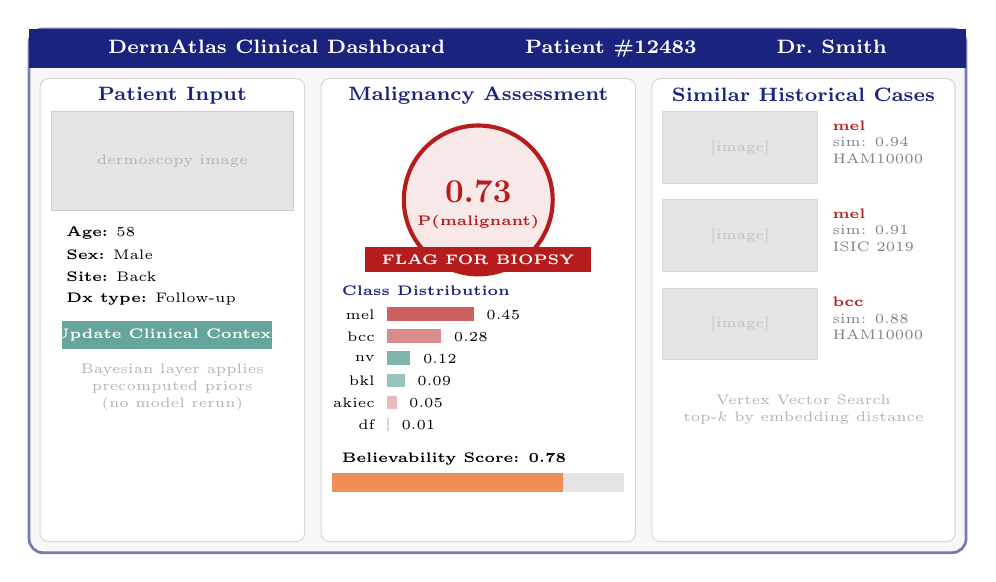
\begin{tikzpicture}[scale=0.70, font=\tiny]

    %% ── Dashboard outer frame ─────────────────────────────────────────────
    \draw[rounded corners=5pt, fill=gray!6, draw=navyblue!60, line width=1pt]
      (0,0) rectangle (17, 9.5);

    %% Title bar
    \fill[navyblue] (0, 8.8) rectangle (17, 9.5);
    \node[white, font=\scriptsize\bfseries] at (8.5, 9.15)
      {DermAtlas Clinical Dashboard \hspace{0.8cm} Patient \#12483
       \hspace{0.8cm} Dr.\ Smith};

    %% ═══ Panel 1: Patient Input ═══════════════════════════════════════════
    \draw[fill=white, rounded corners=3pt, draw=gray!30]
      (0.2, 0.2) rectangle (5.0, 8.6);
    \node[navyblue, font=\scriptsize\bfseries] at (2.6, 8.3) {Patient Input};

    %% Image placeholder
    \fill[gray!20] (0.4, 6.2) rectangle (4.8, 8.0);
    \draw[gray!40] (0.4, 6.2) rectangle (4.8, 8.0);
    \node[gray!60] at (2.6, 7.1) {dermoscopy image};

    %% Clinical fields
    \node[anchor=west] at (0.5, 5.8) {\textbf{Age:} 58};
    \node[anchor=west] at (0.5, 5.4) {\textbf{Sex:} Male};
    \node[anchor=west] at (0.5, 5.0) {\textbf{Site:} Back};
    \node[anchor=west] at (0.5, 4.6) {\textbf{Dx type:} Follow-up};

    \fill[teal!60] (0.6, 3.7) rectangle (4.4, 4.2);
    \node[white, font=\tiny\bfseries] at (2.5, 3.95) {Update Clinical Context};

    \node[gray!60, align=center] at (2.6, 3.0)
      {Bayesian layer applies\\precomputed priors\\(no model rerun)};

    %% ═══ Panel 2: Malignancy Assessment ═══════════════════════════════════
    \draw[fill=white, rounded corners=3pt, draw=gray!30]
      (5.3, 0.2) rectangle (11.0, 8.6);
    \node[navyblue, font=\scriptsize\bfseries] at (8.15, 8.3)
      {Malignancy Assessment};

    %% Score circle
    \fill[darkred!10] (8.15, 6.4) circle (1.35);
    \draw[darkred, line width=1.5pt] (8.15, 6.4) circle (1.35);
    \node[darkred, font=\large\bfseries] at (8.15, 6.55) {0.73};
    \node[darkred, font=\tiny\bfseries] at (8.15, 6.0) {P(malignant)};

    %% Decision flag
    \fill[darkred] (6.1, 5.1) rectangle (10.2, 5.55);
    \node[white, font=\tiny\bfseries] at (8.15, 5.32) {FLAG FOR BIOPSY};

    %% Class distribution bars
    \node[navyblue, font=\tiny\bfseries, anchor=west] at (5.5, 4.75)
      {Class Distribution};

    % bars: left edge at 6.5, max bar width = 3.5 (for prob 1.0)
    \fill[darkred!70]  (6.5,4.2)  rectangle (8.075,4.45); % mel 0.45
    \node[anchor=east] at (6.45,4.32) {mel};
    \node[anchor=west] at (8.12,4.32) {0.45};

    \fill[darkred!50]  (6.5,3.8)  rectangle (7.48,4.05);  % bcc 0.28
    \node[anchor=east] at (6.45,3.92) {bcc};
    \node[anchor=west] at (7.53,3.92) {0.28};

    \fill[teal!50]     (6.5,3.4)  rectangle (6.92,3.65);  % nv 0.12
    \node[anchor=east] at (6.45,3.52) {nv};
    \node[anchor=west] at (6.97,3.52) {0.12};

    \fill[teal!40]     (6.5,3.0)  rectangle (6.815,3.25); % bkl 0.09
    \node[anchor=east] at (6.45,3.12) {bkl};
    \node[anchor=west] at (6.87,3.12) {0.09};

    \fill[darkred!30]  (6.5,2.6)  rectangle (6.675,2.85); % akiec 0.05
    \node[anchor=east] at (6.45,2.72) {akiec};
    \node[anchor=west] at (6.72,2.72) {0.05};

    \fill[teal!20]     (6.5,2.2)  rectangle (6.535,2.45); % df 0.01
    \node[anchor=east] at (6.45,2.32) {df};
    \node[anchor=west] at (6.58,2.32) {0.01};

    %% Believability bar
    \node[font=\tiny\bfseries, anchor=west] at (5.5, 1.7)
      {Believability Score: \textbf{0.78}};
    \fill[gray!20]   (5.5, 1.1) rectangle (10.8, 1.45);
    \fill[orange!65] (5.5, 1.1) rectangle (9.69, 1.45); % 0.78 of width

    %% ═══ Panel 3: Similar Cases ════════════════════════════════════════════
    \draw[fill=white, rounded corners=3pt, draw=gray!30]
      (11.3, 0.2) rectangle (16.8, 8.6);
    \node[navyblue, font=\scriptsize\bfseries] at (14.05, 8.3)
      {Similar Historical Cases};

    % Case 1
    \fill[gray!20] (11.5, 6.7) rectangle (14.3, 8.0);
    \draw[gray!30] (11.5, 6.7) rectangle (14.3, 8.0);
    \node[gray!50] at (12.9, 7.35) {[image]};
    \node[darkred, font=\tiny\bfseries, anchor=west] at (14.4, 7.75) {mel};
    \node[gray,    anchor=west] at (14.4, 7.45) {sim: 0.94};
    \node[gray,    anchor=west] at (14.4, 7.15) {HAM10000};

    % Case 2
    \fill[gray!20] (11.5, 5.1) rectangle (14.3, 6.4);
    \draw[gray!30] (11.5, 5.1) rectangle (14.3, 6.4);
    \node[gray!50] at (12.9, 5.75) {[image]};
    \node[darkred, font=\tiny\bfseries, anchor=west] at (14.4, 6.15) {mel};
    \node[gray,    anchor=west] at (14.4, 5.85) {sim: 0.91};
    \node[gray,    anchor=west] at (14.4, 5.55) {ISIC 2019};

    % Case 3
    \fill[gray!20] (11.5, 3.5) rectangle (14.3, 4.8);
    \draw[gray!30] (11.5, 3.5) rectangle (14.3, 4.8);
    \node[gray!50] at (12.9, 4.15) {[image]};
    \node[darkred, font=\tiny\bfseries, anchor=west] at (14.4, 4.55) {bcc};
    \node[gray,    anchor=west] at (14.4, 4.25) {sim: 0.88};
    \node[gray,    anchor=west] at (14.4, 3.95) {HAM10000};

    \node[gray!60, align=center] at (14.05, 2.6)
      {Vertex Vector Search\\top-$k$ by embedding distance};

  \end{tikzpicture}
  \end{center}
\end{frame}

% ═════════════════════════════════════════════════════════════════════════════
% SLIDE 16b — LLM Summarization Layer
% ═════════════════════════════════════════════════════════════════════════════
\begin{frame}{Slide 17 --- Future Direction: LLM Summarization Layer}

  \begin{columns}[T]

    %% ── Left: the problem + idea ─────────────────────────────────────────────
    \begin{column}{0.44\textwidth}
      \textbf{\color{navyblue}The Cognitive Load Problem}

      \vspace{0.3em}
      {\small
      The physician currently receives three separate outputs
      and must mentally synthesize them:
      \begin{itemize}[leftmargin=1em, itemsep=2pt]
        \item MLP 6-class probability distribution
        \item XGBoost P(malignant) + biopsy flag
        \item Top-$k$ similar historical cases
      \end{itemize}
      }

      \vspace{0.4em}
      \begin{block}{Proposed Addition}
        \small
        A lightweight LLM layer that receives \textbf{all model
        outputs} --- probabilities, cohort deviation scores,
        similar cases, patient metadata --- and generates a
        concise \textbf{clinical narrative} the physician can
        act on immediately.
      \end{block}

      \vspace{0.3em}
      {\scriptsize\color{gray}
      The LLM does not make any clinical decision.\\
      It reduces the cognitive load of reading raw numbers.}
    \end{column}

    %% ── Right: example output + conflict detection ───────────────────────────
    \begin{column}{0.52\textwidth}
      \textbf{\color{navyblue}Example LLM Output}

      \vspace{0.3em}
      \begin{exampleblock}{}
        \scriptsize
        \textit{``This lesion shows strong melanoma
        characteristics (45\%) with notable BCC overlap (28\%).
        The malignancy score of 0.73 exceeds the clinical
        threshold. Cohort deviation is elevated --- this lesion
        looks significantly different from the 847 benign back
        lesions in similar patients, with the closest benign
        neighbor still 0.21 away. Three visually similar
        historical cases were retrieved: two confirmed melanoma,
        one BCC. \textbf{Recommend biopsy.}''}
      \end{exampleblock}

      \vspace{0.3em}
      \begin{alertblock}{Conflicting Signal Detection}
        \scriptsize
        The LLM can flag when outputs disagree --- e.g.\
        \textit{``MLP shows moderate nevus probability (12\%)
        which conflicts with the elevated cohort deviation
        score. Warrants careful review.''}\\[0.3em]
        This is where LLM reasoning adds value beyond
        summarization --- catching ambiguous cases before
        they reach the physician.
      \end{alertblock}

      \vspace{0.2em}
      {\scriptsize\color{gray}
      Context fed to LLM: MLP probs · XGBoost score · knn\_min\_dist
      · lof\_score · top-$k$ case labels · age / sex / site}
    \end{column}

  \end{columns}
\end{frame}

% ═════════════════════════════════════════════════════════════════════════════
% SLIDE 16c — Bayesian Update Layer
% ═════════════════════════════════════════════════════════════════════════════
\begin{frame}{Slide 18 --- Future Direction: Bayesian Clinical Context Layer}

  \begin{columns}[T]

    %% ── Left: concept + formula ──────────────────────────────────────────────
    \begin{column}{0.42\textwidth}
      \textbf{\color{navyblue}The Problem}

      \vspace{0.2em}
      {\small
      The MLP sees only the image. It has no idea whether the
      patient is 25 or 75, male or female. A 25-year-old female
      and a 68-year-old male can produce the \textbf{same MLP
      output} --- but the clinical reality is very different.
      }

      \vspace{0.4em}
      \textbf{\color{navyblue}The Fix: Bayesian Update}

      \vspace{0.2em}
      {\small
      After the MLP produces its 6-class probabilities, the
      physician enters clinical context. A precomputed prior
      table --- $P(\text{class} \mid \text{age, sex, site})$
      --- shifts the distribution without rerunning any model:
      }

      \vspace{0.3em}
      \begin{block}{Formula}
        \small
        \[
          P_c^{\text{updated}} =
          \frac{P_c^{\text{MLP}} \;\times\; P(\text{class}_c \mid \text{context})}
               {\displaystyle\sum_j P_j^{\text{MLP}} \times P(\text{class}_j \mid \text{context})}
        \]
        {\scriptsize Multiply each class score by its demographic
        prior, then renormalise to sum to 1.}
      \end{block}
    \end{column}

    %% ── Right: worked example ────────────────────────────────────────────────
    \begin{column}{0.54\textwidth}
      \textbf{\color{navyblue}Same Image --- Two Patients}

      \vspace{0.3em}
      {\scriptsize MLP output (image only):
      mel=0.45 · nv=0.12 · bcc=0.28 · akiec=0.05 · bkl=0.09 · df=0.01}

      \vspace{0.4em}
      {\small
      \begin{tabular}{@{} l r r @{}}
        \toprule
        Class & \textbf{Patient A} & \textbf{Patient B} \\
              & {\scriptsize 25F · face} & {\scriptsize 68M · back} \\
        \midrule
        {\color{darkred}mel}   & 0.45 $\to$ \textbf{0.14} & 0.45 $\to$ \textbf{0.56} \\
        {\color{teal}nv}       & 0.12 $\to$ \textbf{0.50} & 0.12 $\to$ \textbf{0.08} \\
        {\color{darkred}bcc}   & 0.28 $\to$ \textbf{0.22} & 0.28 $\to$ \textbf{0.27} \\
        {\color{darkred}akiec} & 0.05 $\to$ \textbf{0.04} & 0.05 $\to$ \textbf{0.06} \\
        {\color{teal}bkl}      & 0.09 $\to$ \textbf{0.09} & 0.09 $\to$ \textbf{0.03} \\
        {\color{teal}df}       & 0.01 $\to$ \textbf{0.01} & 0.01 $\to$ \textbf{0.00} \\
        \midrule
        \textbf{P(malignant)}  & 0.73 $\to$ \textcolor{teal}{\textbf{0.40}} & 0.73 $\to$ \textcolor{darkred}{\textbf{0.89}} \\
        \textbf{Decision}      & \textcolor{teal}{watch} & \textcolor{darkred}{biopsy} \\
        \bottomrule
      \end{tabular}
      }

      \vspace{0.3em}
      {\scriptsize\color{gray}
      Patient A: melanoma is rare in young females on the face ---
      prior pulls mel down, nv up.\\
      Patient B: melanoma is common in older males on the back ---
      prior reinforces mel, raises overall malignancy score.\\[0.3em]
      No model reruns. The prior table is precomputed from training data.}
    \end{column}

  \end{columns}
\end{frame}

% ═════════════════════════════════════════════════════════════════════════════
% SLIDE 15 — Limitations & Future Work
% ═════════════════════════════════════════════════════════════════════════════
\begin{frame}{Slide 19 --- Limitations \& Future Work}

  \begin{columns}[T]

    %% ── Left: known limitations ─────────────────────────────────────────────
    \begin{column}{0.52\textwidth}
      \begin{alertblock}{Known Limitations}
        \small
        \begin{itemize}[leftmargin=1em, itemsep=0pt]
          \item \textbf{Class scarcity} --- df: 239 samples, akiec: 1,064.
                Even with inverse-frequency weights, rare class accuracy is limited.
          \item \textbf{Skin tone bias} --- all three datasets are predominantly
                light-skinned European/Australian patients.
                The cohort deviation reference pool inherits this bias.
          \item \textbf{General-purpose embedding} ---
                \texttt{multimodalembedding@001} trained on internet images,
                not dermoscopy. May miss blue--white veils, pigment networks,
                regression areas.
          \item \textbf{ISIC 2020 overlap} --- image sources shared with ISIC 2019;
                potential near-duplicates across datasets.
          \item \textbf{Dropped classes} --- vasc (vascular lesions) and scc
                (squamous cell carcinoma) excluded due to insufficient samples.
        \end{itemize}
      \end{alertblock}
    \end{column}

    %% ── Right: future work ──────────────────────────────────────────────────
    \begin{column}{0.44\textwidth}
      \begin{block}{Future Work}
        \small
        \begin{itemize}[leftmargin=1em, itemsep=0pt]
          \item \textbf{Domain-specific embeddings} --- evaluate SkinGPT or
                DermFoundation backbone; expected to improve rare-class recall.
          \item \textbf{Skin tone auditing} --- collect or synthesize Fitzpatrick
                III--VI examples; measure per-stratum recall.
          \item \textbf{Vector Search deployment} --- build Vertex AI index for
                top-$k$ similar case retrieval in the physician UI.
          \item \textbf{Bayesian update layer} --- precompute
                $P(\text{class}\mid\text{age, sex, site})$ table for interactive
                clinical context adjustment.
          \item \textbf{Believability score} --- classifier confidence
                $\times$ neighbor label agreement for physician trust calibration.
        \end{itemize}
      \end{block}
    \end{column}

  \end{columns}
\end{frame}

% SLIDES 16 AND 17 REMOVED
\end{document}

% ═════════════════════════════════════════════════════════════════════════════
% SLIDE 16 — Physician Feedback Loop (removed)
% ═════════════════════════════════════════════════════════════════════════════
\begin{frame}{Slide 16 --- Physician Feedback: Teaching the Model Over Time}

  \begin{columns}[T]

    %% ── Left: offline retraining ─────────────────────────────────────────────
    \begin{column}{0.32\textwidth}
      \begin{block}{Approach 1 --- Offline Retraining}
        \scriptsize
        \textbf{How it works:}\\
        Physician flags a wrong prediction
        (e.g.\ ``model said benign, biopsy confirmed melanoma'').
        Correction is logged to a feedback database.
        Periodically --- weekly or monthly --- XGBoost and MLP
        are retrained on original data + feedback cases,
        with feedback rows upweighted.

        \vspace{0.3em}
        \textbf{Bayesian connection:}\\
        The prior table $P(\text{class} \mid \text{age, sex, site})$
        is recomputed from the expanded dataset. If a clinic
        sees unusually high melanoma rates in older males,
        that prior shifts --- adjusting every future prediction
        for that demographic before the image is even analyzed.

        \vspace{0.3em}
        \textbf{Pros:} Simple, safe, stable.\\
        \textbf{Cons:} Model only improves on next deployment cycle.
      \end{block}
    \end{column}

    %% ── Middle: online reranking ─────────────────────────────────────────────
    \begin{column}{0.34\textwidth}
      \begin{alertblock}{Approach 2 --- Online Reranking Layer}
        \scriptsize
        \textbf{How it works:}\\
        A lightweight layer sits \textit{on top} of XGBoost.
        The base model score is fixed. The reranker adjusts it
        up or down in near real-time based on patterns learned
        from physician overrides --- without touching the
        underlying model.

        \vspace{0.3em}
        \textbf{Bayesian framing:}
        \[
          P(M \mid \text{img, feedback})
        \]
        \[
          \propto \underbrace{P(\text{fb} \mid M)}_{\text{reranker}}
          \times \underbrace{P(M \mid \text{img})}_{\text{XGBoost}}
        \]
        If physicians at a clinic consistently override the model
        for lesions on darker skin, the reranker learns that
        correction and applies it to similar future cases
        automatically.

        \vspace{0.2em}
        \textbf{Pros:} Near real-time improvement.\\
        \textbf{Cons:} Risk of drift if feedback is noisy.
      \end{alertblock}
    \end{column}

    %% ── Right: how they compose ──────────────────────────────────────────────
    \begin{column}{0.30\textwidth}
      \textbf{\color{navyblue}How All Three Compose}

      \vspace{0.3em}
      {\scriptsize
      \begin{tabular}{@{} p{2.6cm} @{}}
        \toprule
        \textbf{Base XGBoost score}\\
        $P(M \mid \text{image})$\\
        \midrule
        $\times$\; \textbf{Clinical prior}\\
        $P(\text{class} \mid \text{age, sex, site})$\\
        Updates from offline retraining\\
        \midrule
        $\times$\; \textbf{Feedback correction}\\
        $P(\text{feedback} \mid M)$\\
        Learned from physician overrides\\
        \midrule
        $=$ \textbf{Final calibrated score}\\
        \bottomrule
      \end{tabular}
      }

      \vspace{0.3em}
      {\scriptsize\color{gray}
      Three multiplicative factors, each adding
      a different type of knowledge:
      \begin{itemize}[leftmargin=1em, itemsep=0pt]
        \item Visual (XGBoost)
        \item Demographic (prior table)
        \item Experiential (feedback reranker)
      \end{itemize}
      The current system has the first two.
      The reranking layer is the natural next step.
      }
    \end{column}

  \end{columns}
\end{frame}

% ═════════════════════════════════════════════════════════════════════════════
% SLIDE 17 — Industry Comparison
% ═════════════════════════════════════════════════════════════════════════════
\begin{frame}{Slide 17 --- How We Compare to Industry}

  \begin{columns}[T]

    %% ── Left: where we are on par ────────────────────────────────────────────
    \begin{column}{0.48\textwidth}
      \begin{exampleblock}{Where We Are On Par}
        \scriptsize
        \begin{itemize}[leftmargin=1em, itemsep=0pt]
          \item \textbf{XGBoost on learned features} --- the same pattern
                used by Google, Meta, and most production ML systems.
                More interpretable and faster to retrain than end-to-end
                deep learning
          \item \textbf{Cohort deviation} --- clinically grounded signal
                most academic pipelines skip. Validated by \texttt{knn\_min\_dist}
                becoming the \#2 most important XGBoost feature
          \item \textbf{Threshold tuning for recall} --- explicitly
                optimizing for the clinical objective rather than default
                $\tau=0.50$. Standard in any serious clinical ML system
          \item \textbf{OOF discipline} --- rigorous leakage prevention
                across pipeline stages; same standard as production deployments
        \end{itemize}
      \end{exampleblock}
    \end{column}

    %% ── Right: where industry is ahead ──────────────────────────────────────
    \begin{column}{0.48\textwidth}
      \begin{alertblock}{Where Industry Is Ahead}
        \scriptsize
        \begin{itemize}[leftmargin=1em, itemsep=0pt]
          \item \textbf{End-to-end fine-tuning} --- industry unfreezes the
                ViT backbone and trains it jointly with the classifier on
                dermoscopy data. Gradients flow all the way back through
                the embedding model, teaching it to encode dermoscopy-specific
                structures (blue-white veils, pigment networks). We cannot
                do this --- \texttt{multimodalembedding@001} is a closed API
          \item \textbf{Domain-specific foundation models} --- Google Health,
                PathAI, Skin Analytics pretrain on millions of clinical images.
                A dermoscopy-specific ViT would close most of our AUC gap
          \item \textbf{Uncertainty quantification} --- industry outputs
                calibrated confidence intervals (``$73\% \pm 12\%$''), not
                point estimates. Requires Bayesian deep learning or
                Monte Carlo dropout
          \item \textbf{Data scale} --- 30,647 labeled images vs.\ millions
                in proprietary clinical datasets
        \end{itemize}
      \end{alertblock}

      \vspace{0.2em}
      {\scriptsize\color{gray}
      Swapping \texttt{multimodalembedding@001} for an open-source
      dermoscopy foundation model (e.g.\ SkinGPT) would close most
      of the gap immediately --- the pipeline architecture is already
      production-grade.}
    \end{column}

  \end{columns}
\end{frame}

\end{document}
